\documentclass[tikz,border=2pt]{standalone}
\usepackage{tikz}
\usepackage{lmodern}
\usetikzlibrary{calc,decorations.pathreplacing}

% Visual conventions follow the existing MRNC TikZ pictures: ordinary
% components use TikZ's normal 0.4pt stroke, with compact TeX labels.
\tikzset{
  nu fibre/.style={
    x=0.78cm,
    y=0.78cm,
    line width=0.4pt,
    line cap=round,
    line join=round
  },
  nu label/.style={
    font=\scriptsize,
    inner sep=1pt
  },
  nu annotation/.style={
    font=\scriptsize,
    inner sep=1pt
  },
  nu dots/.style={
    font=\small,
    inner sep=0pt
  }
}

\begin{document}
% Namikawa--Ueno type VIII-3; NU p. 15.
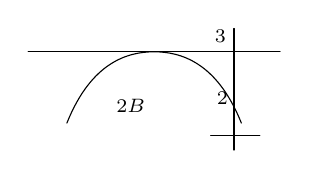
\begin{tikzpicture}[nu fibre]

  \draw (-2.05,0.58) -- (2.05,0.58);
  \node[nu label,above=2pt] at (1.08,0.58) {$3$};

  \draw (-1.42,-0.58) .. controls (-1.02,0.42) and (-0.42,0.58) .. (0,0.58)
                         .. controls (0.42,0.58) and (1.02,0.42) .. (1.42,-0.58);
  \node[nu label] at (-0.38,-0.30) {$2B$};

  \draw (1.30,-1.02) -- (1.30,0.96);
  \node[nu label,left=1pt] at (1.30,-0.18) {$2$};
  \draw (0.92,-0.78) -- (1.72,-0.78);

\end{tikzpicture}
\end{document}
